% il existe plusieures classes de documents
% pour des documents plus longs, vous pouvez utiliser
% book ou report
\documentclass[a4paper]{article} 



% vous pouvez changer les paramètres : voici les options dispoinibles :
% - a4paper
% - fancysections
% - notitlepage ou titlepage
% - onside ou twoside selon si vous voulez l'imprimer en recto-verso ou en recto
% - sectionmark
% - chaptermark (pour les 
% - pagenumber
% - enmanquedinspiration
% en cas de doutes, pas de doutes, la documentation est sur :
% https://gitlab.binets.fr/typographix/polytechnique/-/blob/master/source/polytechnique.pdf
\usepackage[a4paper, fancysections, titlepage]{polytechnique}
\usepackage[french]{babel}
\usepackage[T1]{fontenc}
\usepackage{blindtext}
\usepackage[hidelinks]{hyperref}
\usepackage{amsmath, amssymb}

% nous avons défini deux commandes :
\newcommand{\code}[1]{%
\mbox{\ttfamily%
\detokenize{#1}%
}%
}

\newcommand{\resultat}[1]{%
\quad \rightsquigarrow \quad #1%
}

\author{Mathias \textsc{Ollu}, Juliette \textsc{Anglade}, Alexandre \textsc{Parvery}, Albert \textsc{Moulin}}
\date{27 septembre 2024}
\title{Proposition Détaillé}
\subtitle{
Projet scientifique collectif
}
% pour changer de logo, ajoutez l'image dans un fomat PDF
% ou image en la glissant à droite et remplacez typographix
% par le nom de l'image, si vous ne voulez pas de logo, 
% supprimze la ligne. 
% navy ou cmd ducuing



\begin{document}
\maketitle 
% saut de page
\vfill
\Large
\tableofcontents
\newpage


\section{Contexte et objectif du projet}



“If you owe the bank a hundred thousand dollars, the bank owns you. If you owe the bank a hundred million dollars, you own the bank”. Ce proverbe américain figurant en introduction de Debt : the first 5.000 years (2011) de l’anthropologue David Graeber est une description à notre sens fidèle de l’état de la dette publique française aujourd’hui. 

D’un côté, l’Etat a échoué de manière répétitive à redresser la trajectoire de ses déficits chroniques, avec un déficit prévu de l’ordre de 6% de Produit Intérieur Brut (PIB) en 2024 (AFT, 2014). Régulièrement, le risque d’une augmentation rapide des taux d’intérêts pour la soutenabilité de la dette est mentionné dans le débat public, et donne l’impression que l’Etat, et par extension le pays, sont à la merci d’un changement d’humeur des marchés financiers. 
De l’autre côté, l’effet de ce surendettement de 110,4% du PIB, le troisième plus élevé d’Europe (INSEE, 2024), n’est que peu sensible pour le moment. La France s’endette à des taux proches de ceux de l’Allemagne, référence en termes de stabilité financière, avec un spread sous le demi-point de base durant l’essentiel des dix dernières années (Boursorama, 2024), et elle ne semble pas rencontrer de difficultés majeures à lever environ 300 milliards d’euros par an depuis 2022 sur les marchés (AFT, 2024). 

Cette situation, d’apparence paradoxale, est le résultat d’un contexte macro-financier bien particulier, caractérisé notamment par la confiance des marchés en la monnaie européenne, le demande renforcée de valeurs sûres, dont la dette française fait encore partie, par les investisseurs institutionnels suite au renforcement de la régulation financière depuis 2008 (cf source), et par les anticipations faibles de l’inflation et des intérêts à long terme. 

Ayant assisté à la conférence co-organisée par l’Ecole Polytechnique et la Cour des Comptes le 15 mai 2024, notre groupe a acquis la conviction que la dette publique est déterminée par l’intrication de facteurs purement financiers, économiques, politiques et démographiques, tant français qu’européens. C’est bien cette interaction qui nous fascine, et qui nous semble cristallisée dans la courbe des rendements sur les titres souverains.

L’évolution de cette courbe, c’est-à-dire le taux d’intérêt sur une obligation souveraine française en fonction du temps et de la maturité, est l’un des indicateurs cruciaux décrivant la situation financière de l’Etat. C’est cette courbe qui détermine à quel prix celui-ci s’endette, et à quelle maturité il peut le faire - c’est-à-dire à quel point il peut se projeter dans le futur. Elle détermine sa solvabilité, des taux trop élevés empêchant l’Etat de faire rouler sa dette existante. Elle reflète également les anticipations des acteurs économiques en matière de croissance, d’inflation ou encore de politiques publiques. Enfin, la dette souveraine française étant un actif sûr, elle détermine la façon dont les acteurs économiques valorisent l’avenir.

En ce sens, il nous a semblé que comprendre les mécanismes sous-jacents de la courbe de rendement sur l’emprunt public constitue l’une des clés pour appréhender le fonctionnement de l’économie française en général, la marge de manœuvre de l’Etat, et le fonctionnement des marchés financiers. 

Nous avons donc décidé de consacrer notre PSC à l’étude d’un modèle à cascade stochastique proposé par Laurent-Emmanuel Calvet, Fisher et Wu dans leur article Staying on Top of the Curve: A cascade Model of Term Structure Dynamics de Calvet, Fisher et Wu (2018), conçu pour la modélisation de la courbe de rendement d'obligations privées. L’intérêt de notre étude consiste en l’adaptation de ce modèle aux obligations souveraines françaises - que ce soit par la prise en compte de facteurs spécifiques à la dette publique, ou par la modification de certaines propriétés du modèle afin qu’il simule plus fidèlement certains mécanismes propres aux obligations souveraines.

L’intérêt majeur de ce modèle est son aspect multifractal, découlant de la cascade stochastique, qui permet de modéliser une fluctuation des taux hétérogène dans le temps, ainsi que des réactions aux chocs macroéconomiques, politiques ou financiers qui diffèrent selon les maturités. Étant non-paramétrique, ce modèle ne suppose pas de forme a priori de la courbe des rendements, lui conférant une plus grande flexibilité qui pourrait être utile pour son adaptation à un type d’actifs nouveaux.

Nos premiers résultats (cf Partie 6) semblent indiquer que la courbe des rendements sur la dette publique française est caractérisée par des dynamiques très hétérogènes dans le temps et la maturité, en particulier au cours de l’été 2024 et la crise politique qui l’a marqué. Ainsi, il nous apparaît qu’un enjeu fondamental de notre PSC sera de parvenir à capturer les différentes échelles de temps en jeu, de un mois à trente ans, dans la détermination des taux.

Enfin, ce modèle nous paraît particulièrement adapté du fait de son emphase sur le long terme. L’Etat est en effet un créancier caractérisé par sa longue durée de vie, voir son immortalité, et donc essentiellement par des enjeux de long terme. L’émission récente d’obligations assimilables au trésor de 50 ans en témoigne. Il nous a donc semblé essentiel de partir d’un modèle qui vise avant tout à modéliser les taux sur des maturités élevées.

Nous avons d’ores et déjà en tête certains facteurs dont nous pensons qu’il pourrait être envisageable d’étudier les effets. Le premier concerne les effets des nouvelles économiques et leur anticipation ou non par les marchés. Un exemple serait l’annonce d’un déficit plus élevé que prévu. Nous pensons aussi à capturer l’effet classique de la politique monétaire avec les anticipations d’inflation et de croissance. Il serait également intéressant de comparer l’exposition des rendements français à des facteurs purement nationaux avec des facteurs européens.
La forme particulière de la courbe des rendements de la dette publique française nous invite également à penser qu’une prise en compte des différentes échelles de temps et en particulier des effets courts termes et longs termes pourrait être également intéressante.

Enfin, l’actualité récente en France a souligné l’importance de la stabilité politique pour la stabilité des taux, alors que ce type de risque est habituellement davantage associé à des pays en voie de développement. Si il est difficile de modéliser quantitativement des facteurs politiques, nous pourrions tenter de prendre en compte une représentation sophistiquée de la politique budgétaire. Elle inclurait bien sûr le déficit, mais aussi par exemple le déficit dédié à des dépenses courantes (au lieu d’investissements), ou la différence entre le déficit public et la croissance. En effet, ces facteurs pourraient refléter un contexte politique défavorable à une politique budgétaire équilibrée. Un gouvernement qui maintient des déficits élevés en période de croissance peut par exemple être perçu comme peu engagé pour la stabilité budgétaire, tout comme un gouvernement qui ferait exploser les dépenses courantes en les finançant par de la dette.

Ceci n’est qu’une première liste de possibilités, elle n’a pas vocation à être exhaustive. De plus, des questions portant sur l’évaluation et la modélisation de tels facteurs se posent et nous espérons que notre travail pourra apporter des éléments de réponse.
\newpage

\section{Etat de l’art}


L’intérêt majeur de notre étude réside dans le constat que si la littérature économique et financière est abondante sur les questions de modélisation de courbes de rendement du secteur privé, nous n’avons pas encore trouvé de modèle spécifique à la dette publique. 

… Modèle Heath Jarrow Morton A COMPLETER

Par ailleurs, il nous semblerait intéressant d’étudier les modèles qu’utilise l’Agence France Trésor, l’agence publique semi indépendante en charge de la gestion de la dette publique française sur les marchés. Selon nos recherches, elle n’utilise pas non plus de modèle spécifique aux taux souverains (cf Partie 5).




\section{Objectifs intermédiaires}



Afin de mener à bien ce projet, nous avons défini une feuille de route destinée dans un premier temps à nous permettre d’appréhender le sujet, à la fois sous ses aspects mathématiques et économiques. 

Notre point de départ est l’article Staying on Top of the Curve: A cascade Model of Term Structure Dynamics de Calvet, Fisher et Wu (2018), qui met à plat le modèle que nous devrons étudier, modifier et appliquer à notre sujet d’étude. Sa compréhension entière nécessite à notre sens un temps d’étude des grands principes d’économie et de finance qui régissent la théorie et les méthodes de l’asset pricing - dont le principe de non arbitrage et ses implications, le rôle des probabilités neutres au risque, ainsi que les principes de modélisation des facteurs considérés dans un modèle en finance. Il nous faut également préciser notre compréhension des mathématiques sous-tendant le modèle, en particulier en étudiant les preuves des résultats du papier détaillées dans des travaux antérieurs, dont la représentation factorielle du taux d’intérêt immédiat, ou encore les résultats de convergence de la structure taux d’intérêts à long terme. A cet effet, nous comptons nous appuyer sur des cours de mathématiques financières et d’économie éventuellement fournis par M. Calvet, ainsi que sur des papiers antérieurs.

En parallèle, nous souhaitons creuser davantage notre sujet d’étude final: la courbe des taux d’intérêts de la dette publique française. Ce travail préliminaire est à notre sens indispensable afin de dégager les pistes d’adaptation du modèle à la dette publique. Il doit également nous permettre d’identifier les facteurs essentiels pour la modélisation, ainsi que la période temporelle la plus pertinente à étudier (cf Partie 5).

Nous avons pour objectif de clore cette première partie d’appréhension du sujet mi-novembre, bien que la partie concernant l’étude de la dette publique française et ses enjeux se prolongera au-delà.

Ensuite, notre objectif sera d’être capable de reproduire les résultats du modèle, et éventuellement de l’appliquer naïvement à nos données sur la dette afin d’étudier son comportement. Cette partie nécessitera de coder le modèle informatiquement, en s’appuyant éventuellement sur l’architecture fournie par M. Calvet. Nous anticipons que cette partie, qui semble courte de prime abord, pourrait prendre du temps en raison d’éventuelles difficultées techniques dans l’implémentation du modèle, et notamment pour son application aux données. Nous prévoyons donc qu’elle se termine début février, après quoi nous entendons maîtriser et savoir appliquer le modèle à des données de notre choix.

A cette étape, il nous sera déjà possible de rédiger une partie importante du rapport final de PSC. Nous enchaînerons enfin avec la modification du modèle afin de l’adapter à la dette publique. La plus grande difficulté sera ici à notre sens de modéliser l’effet d’annonces politiques ou économiques particulièrement importantes dans le cas de la dette publique. Par exemple, la dégradation de la note de la dette française par l’agence Standard \& Poors n’a que très peu affecté les taux souverains en raison de l’anticipation de celle-ci par les marchés, tandis que l’annonce des déficits record de l’années 2024, pourtant prévisibles, a affecté plus durement les cours. Il nous faudra donc sélectionner finement les nouveaux facteurs pris en compte par le modèle. Nous anticipons donc que cette partie verra des allers retours entre la théorie et l’application aux données, selon les performances établies du modèle. Elle s’étendra jusqu’à la fin du PSC, la fin de la rédaction du rapport pouvant s’étaler tout au long de celle-ci.

\section{Méthodologie et organisation du travail et répartition des tâches}
 
Notre sujet de PSC requiert à la fois une bonne compréhension des phénomènes économiques, une très bonne maîtrise des outils mathématiques convoqués ainsi que des compétences en programmation. Nous comptons donc exploiter au mieux la complémentarité des profils qui constituent notre groupe. Nous venons en effet de différentes filières (FUF-maths/éco, MP-info, PC) et avons fait des choix de cours de 2A complémentaires, en économie, processus stochastiques, informatique et statistiques.
 
Néanmoins, nous comptons bien donner à notre travail une dimension éminemment collective.  Ainsi, nous travaillerons ensemble le mercredi. Nous envisageons également -si la situation s’y prête- de nous subdiviser en binômes pour travailler sur certaines tâches en étant plus rapides et donc plus efficaces. Enfin, pour partager nos travaux, réflexions et recherches individuelles, nous avons d’ores et déjà créé un espace de partage de documents et une bibliographie Zotero. Lorsque nous en viendrons à devoir écrire du code, nous créerons un dépôt Git. 
 
Nous rencontrerons régulièrement notre encadrant en visioconférence pour lui poser des questions, faire le bilan de notre avancement, évoquer nos éventuelles difficultés, et obtenir de nouvelles pistes de réflexion. 
\newpage

\section{Contribution de partenaires internes et externes}

Pour la réalisation de notre projet scientifique commun, nous allons avoir besoin de différentes données et de code pour pouvoir appliquer les modèles étudiés. Notre objectif n’est pas seulement d’étudier des modèles mais également de les mettre en pratique pour pouvoir tester de nouvelles méthodes.

La majorité des données à propos de la dette publique et sur l’achat d’obligations sont publiques et aisément accessibles sur internet. Nos sources principales sont la Direction générale du Trésor, la Banque de France et Bloomberg. Sur leurs sites internets respectifs, les données et chiffres de la dette français et américaine peuvent être récupérés pour être traités par nos algorithmes.

La Direction générale du Trésor fait partie du ministère de l’économie et des finances et a pour mission d’analyser l’économie française et internationale, ainsi que d’assister le ministère dans la prise de décision sur la politique économique. Elle étudie notamment la dette publique et ses publications permettent un travail et une étude approfondie et fiable.

La Banque de France est la banque centrale française qui a pour mission d’assurer la stabilité économique et financière de la France comme membre de l’Eurosystème. Elle publie sur son site les différents rendements des obligations souveraines. Ce sont les données de base de notre analyse que nous allons faire dans le but d’appliquer le modèle de Laurent-Emmanuel Calvet.

Bloomberg est une entreprise américaine de services qui donne des informations économiques et financières. Elle fournit donc directement les données sur le cours de la dette. Ces données sont disponibles sur internet, au sein des publications de Bloomberg.   

Nous pourrions également récupérer les algorithmes informatiques utilisés en recherche, dont celui de M. Calvet. Cela nous permettra de comprendre comment des algorithmes sont codés dans le milieu de la finance et de l’économie. Comprendre cette architecture et cette nouvelle façon de penser est essentielles pour produire des algorithmes performants et espérer produire des résultats concluants.

Enfin, comme justifié en partie 2, nous souhaitons contacter l’Agence France Trésor afin d’en apprendre plus sur sa stratégie de modélisation. Cela nous permettrait par ailleurs d’approfondir notre compréhension du processus de mise sur le marché des obligations françaises, et d’enrichir notre réflexion sur les types de facteurs à prendre en compte dans le cas spécifique de la dette publique.




\section{Résultats préliminaires}
\subsection{Les données}


Afin de nous familiariser avec notre objet d’étude, il nous a paru essentiel de pouvoir nous représenter l’évolution de la courbe des rendements de la dette française. La représentation en trois dimensions de l’intérêt en fonction du temps et de la maturité durant l’été 2024 (fig. 1) permet quelques observations clés.
\begin{center}

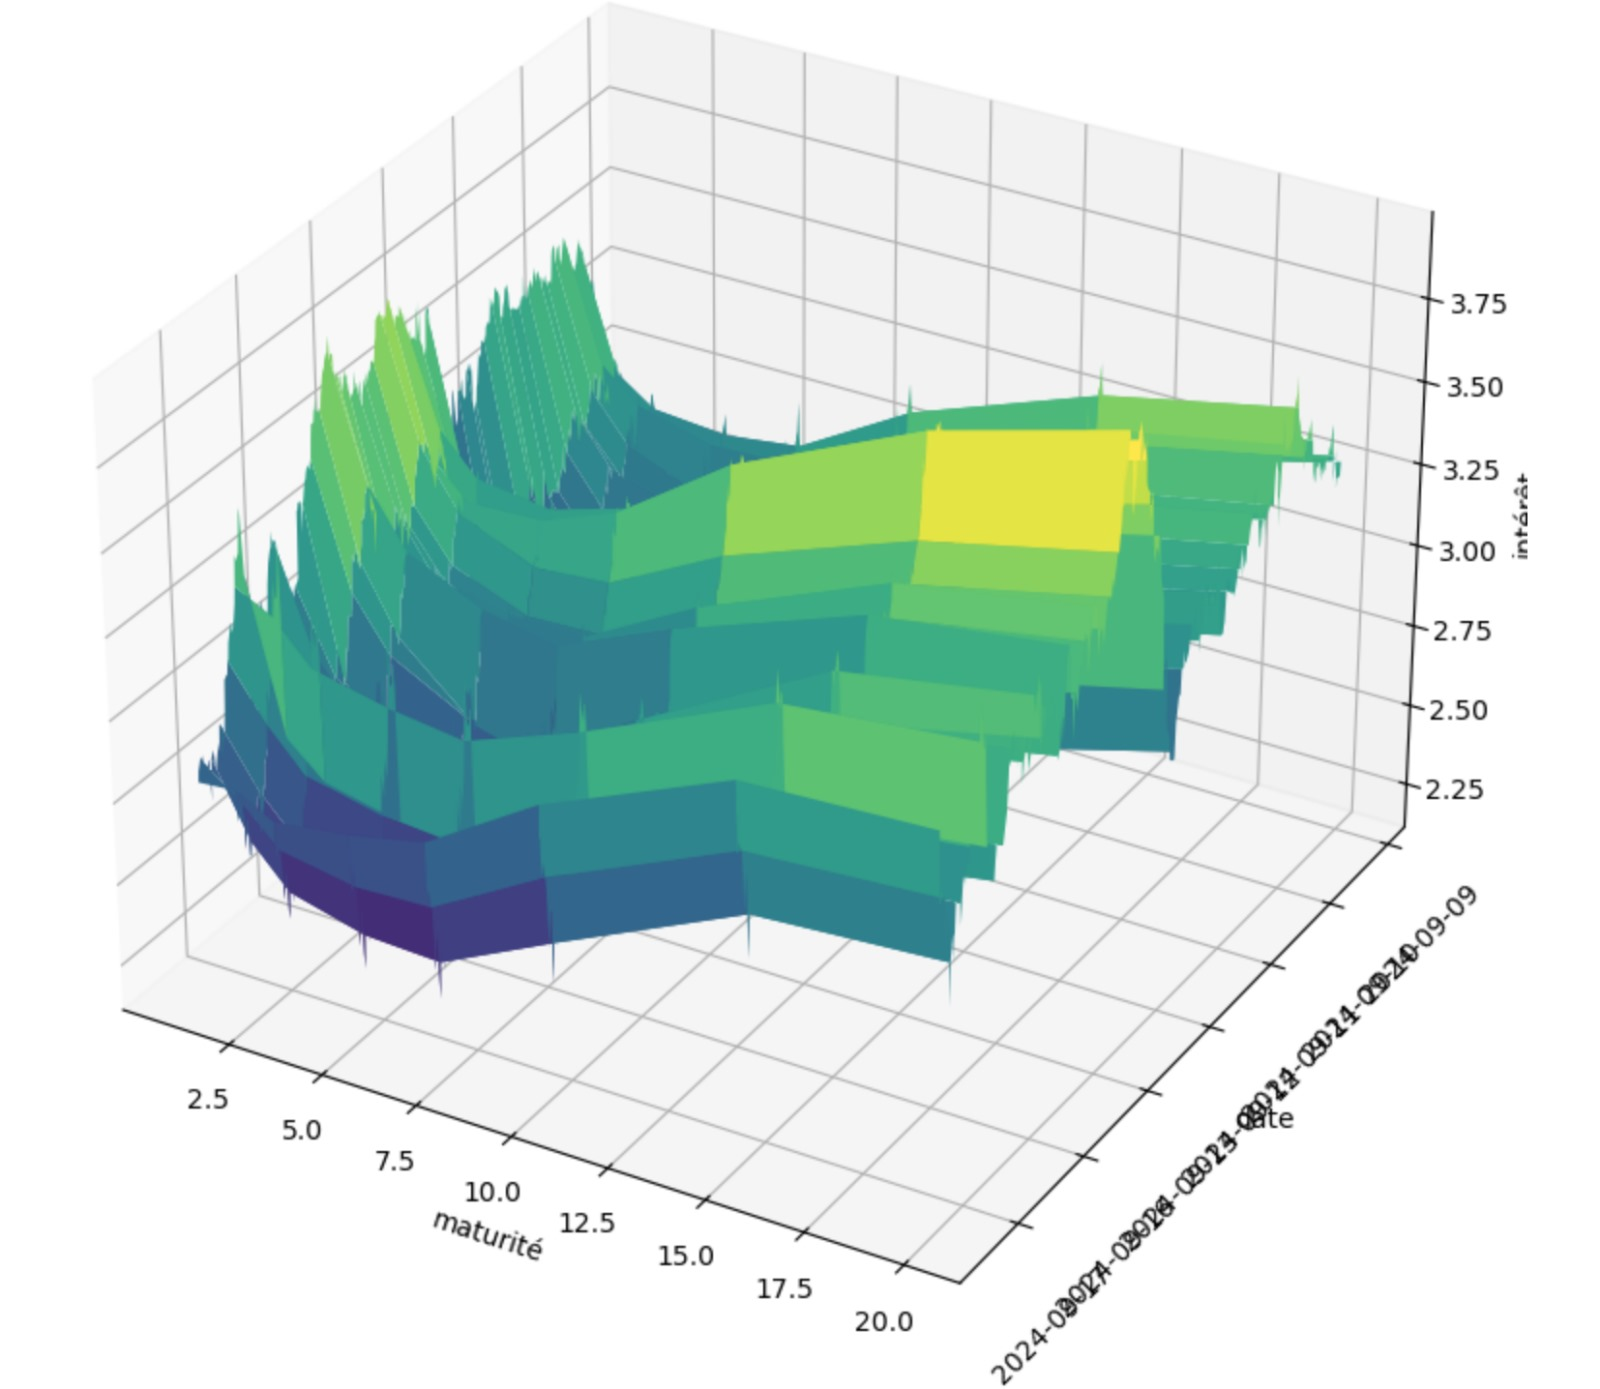
\includegraphics[scale=0.28]{intd.jpg}

Figure 1: Évolution de la courbe des rendements sur les titres souverains français dans le temps, entre le 1er avril et le 18 septembre 2024.
\end{center}



D’abord, la courbe des rendements prend une forme parabolique: le rendement à un an est presque supérieur d’un demi-point de base au taux à deux ans. Il faut considérer des maturités élevées, autour de vingt ans, pour revenir à hauteur du taux de court terme. Ce phénomène très documenté d’inversion de la courbe des rendements est habituellement perçu comme signalant une période de pré-récession, lorsque le risque immédiat est considéré comme supérieur au risque de long terme. On retrouve donc sans doute l’effet de la crise politique et budgétaire actuelle en France. 

Pourtant, le phénomène est à l’œuvre depuis près d’un an, et touche d’autres économies avancées dont l’Allemagne et les Etats-Unis bien qu’à plus faible magnitude. D’autres facteurs sont donc en jeu, et notamment l’anticipation de baisses des taux et d’une décrue de l’inflation à moyen terme malgré des valeurs actuelles élevées qui pourraient provoquer ce déséquilibre entre court et moyen terme (BCE, 2023). On devine donc qu’il sera crucial de modéliser l’effet des anticipations d’inflation, de taux directeur mais aussi de croissance sur plusieurs échelles de temps, comme le permet un modèle multifractal.

Ensuite, on observe une décrue forte des rendements de près d’un demi-point de base sur deux mois, qui semble anticiper la baisse des taux directeurs de la Banque Centrale Européenne du 18 septembre 2024, et ce malgré un contexte budgétaire particulièrement difficile en France. On retrouve donc ici aussi le rôle crucial de la politique monétaire comme facteur de notre modèle.

Enfin, l’étude croisée avec la figure 2 montre la forte volatilité intermittente des rendements à toutes les maturités, en particulier entre mi-mai et mi-juillet 2024. Par la suite, on observe au contraire une décrue très régulière des rendements. Conséquence entre autres de la dissolution de l’Assemblée Nationale, cette volatilité intermittente sera un enjeu central de la modélisation des rendements: sur un intervalle de quinze jours encadrant les deux tours des législatives anticipées du 30 juin et 6 juillet, le rendement à sept ans a connu une variation de près d’un demi-point de base, soit de l’ordre de la variation totale du cours sur trois mois.
\newpage
\begin{center}

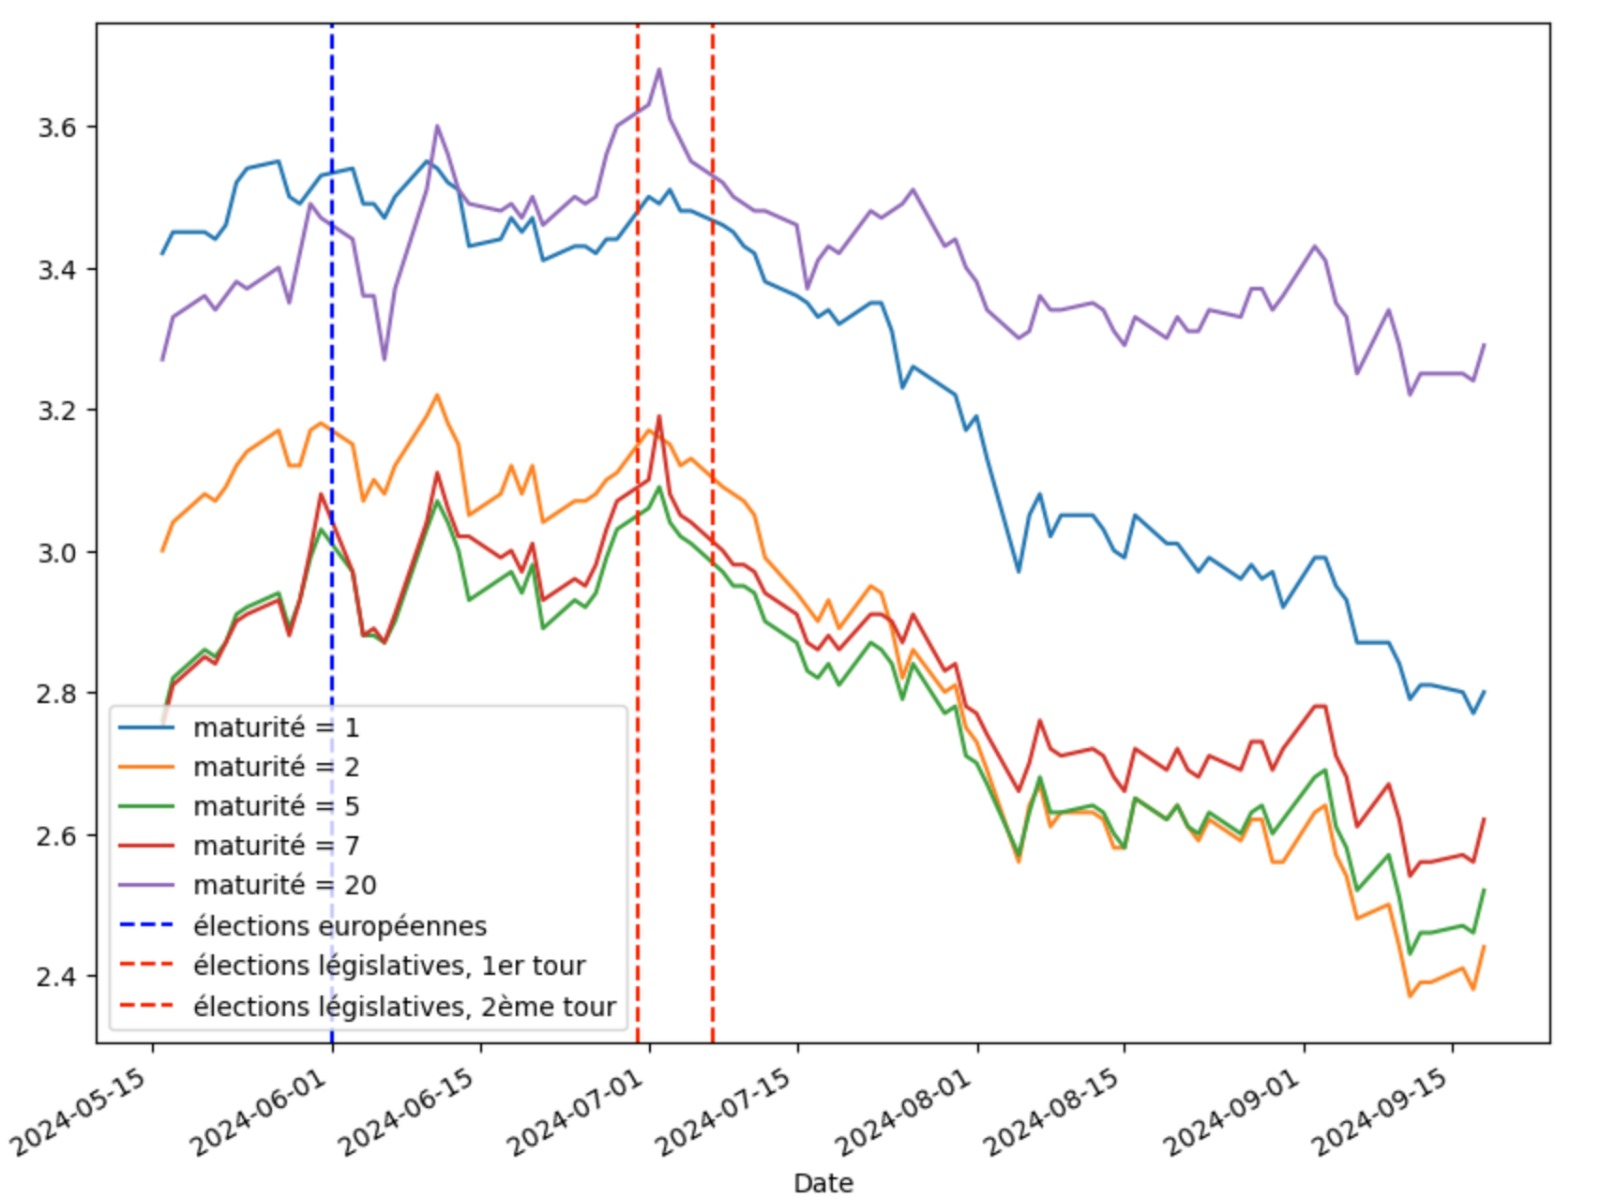
\includegraphics[scale=0.25]{election.jpg}

Figure 2. Rendements des titres souverains français pour différentes maturités, entre le 1er avril et le 18 septembre 2024

\end{center}



On retrouve également l’importance d’une modélisation fine de la volatilité en observant les distributions sur cinq mois et demi des rendements pour différentes maturités. En plus de la volatilité intermittente observée sur la figure 2, on constate en effet des régimes de volatilité très différents entre les différentes maturités, avec une variance élevée des rendements à court et moyen terme. Notre modèle devra donc être capable de rendre compte de ces différents régimes.

\begin{center}


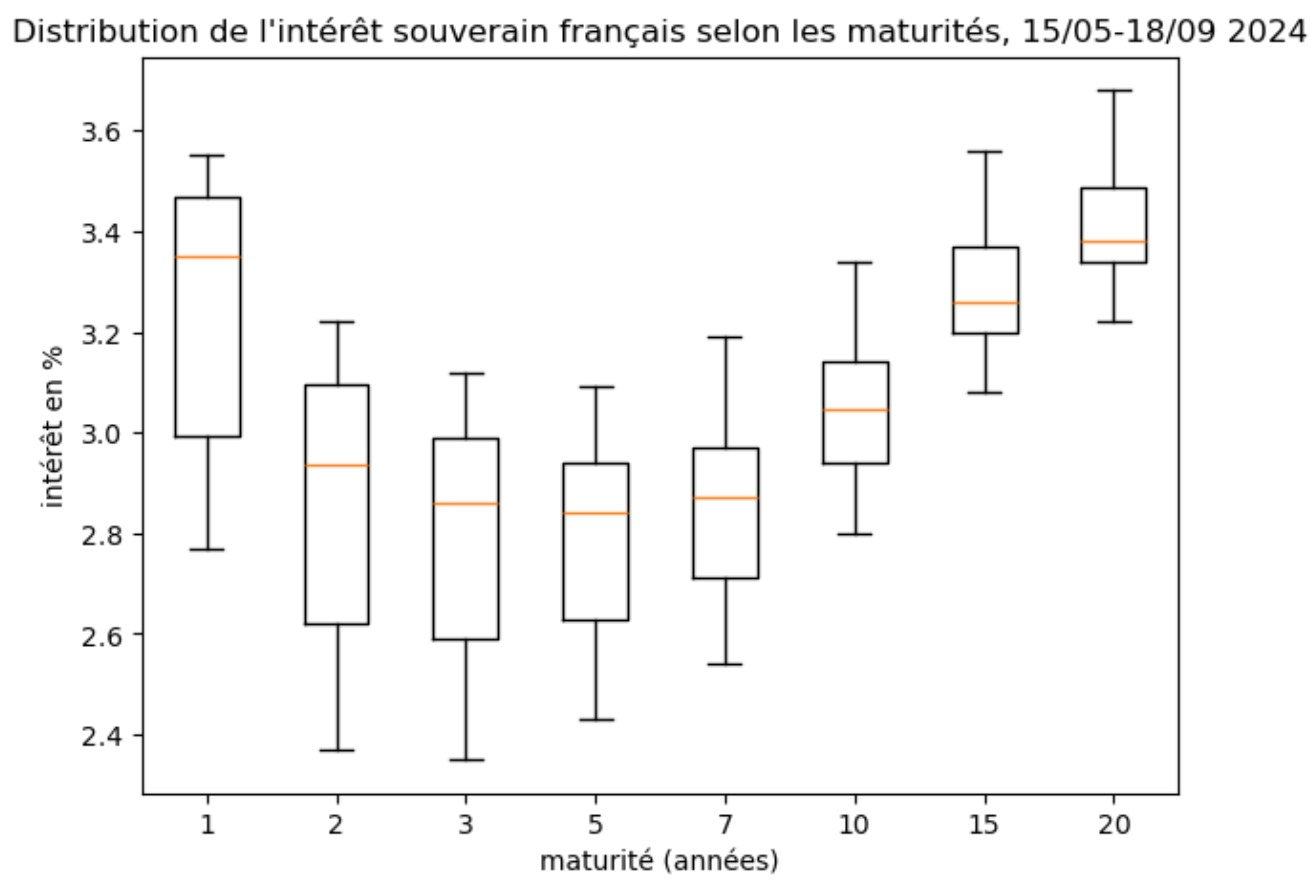
\includegraphics[scale=0.29]{distribution.jpg}

Figure 3: Distribution des rendements sur les titres souverains français, 1er avril au 19 septembre 2024

\end{center}


\subsection{Le modèle}



L’étape suivante fut de lire l'article de M Calvet et de s'approprier son modèle de cascade récursif dans le but de l'appliquer numériquement au marché des obligations sur la dette française. Ce modèle repose donc sur une structure de cascade récursive dictée par l'équation suivante (ici sous forme matricielle) :
$$ d\boldsymbol{X}_t = \boldsymbol\kappa (\boldsymbol\theta - \boldsymbol{X}_t)d_t + \boldsymbol\Sigma^{\frac{1}{2}} d\boldsymbol{W}_t$$
avec $\boldsymbol{X}$ le vecteur d’état, $\boldsymbol{W}$ un processus de Wiener et $\boldsymbol\Sigma$, $\boldsymbol\kappa$ et $\boldsymbol\theta$ des paramètres du modèle. La résolution de cette équation dans le cas général permet ensuite de considérer la solution par rapport à une mesure neutre au risque. L'existence d'une telle mesure repose sur l'hypothèse d'un marché sans arbitrage. Le modèle permet alors d'estimer le taux d'intérêt d'une obligation à coupon zéro et par extension d'estimer son prix pour une maturité donnée. Ce modèle permet avec une dimension limitée du vecteur d’état, optimale pour n (la dimension du vecteur) fixé à 10, de produire des courbes de taux qui correspondent aux données presque parfaitement. Il faudra alors voir si ce modèle permet d'estimer les courbes de taux sur la dette française et s’il peut s'adapter à des perturbations liées au contexte économique et politique du pays.

\section{Références}
\begin{itemize}

\item Agence France Trésor (2024) Budget de l’Etat. \href{https://www.aft.gouv.fr/fr/budget-etat. }{Accessible}

\item Banque de France (2024) Indices obligataires - 2024-09-20. \href{https://www.banque-france.fr/fr/statistiques/taux-et-cours/indices-obligataires-2024-09-20}{Accessible}

\item Banque Centrale Européenne (2023) Bulletin économique - volume 7. \href{https://www.ecb.europa.eu/press/economic-bulletin/focus/2023/html/ecb.ebbox202307_02~78906aa989.en.html }{Accessible}

\item Boursorama. (2024) Taux souverains, zone Europe-Allemagne. \href{ https://www.boursorama.com/bourse/taux/souverains/?area_filter%5Bcountries%5D=DEU }{Accessible}

\item Calvet, L.E., Fisher, A.J., Wu, L. (2018) Staying on Top of the Curve: A cascade Model of Term Structure Dynamics. Journal of financial and quantitative analysis, VOL 53, No.2. pp. 937-963

\item Graeber, D. (2011) Debt, the first 5.000 years., Melville House Publishing.

\item Institut National des Statistiques et des Etudes Economiques. (2024) À la fin du premier trimestre 2024, la dette publique s’établit à 3 159,7 Md€. \href{https://www.insee.fr/fr/statistiques/8210074}{Accessible}.


\end{itemize}

\end{document}
